%%%%%
%%%%% Chapter 3
%%%%%
\chapter{Simple Sampling of Probability distributions Using Random numbers}
This Chapter is devoted to the following question: How can we 
generate sequences of random numbers which are distributed 
according to some given distribution?

A simple answer to this question would be to exploit some 
intrinsically random physical process. For example, one could 
record a sequence of the decay times of some radioactive substance 
and use this truly random sequence of numbers in a Monte--Carlo
simulation. Although tables of millions of such true random 
numbers exist in practice this approach turns out not to be very
practical. Monte--Carlo simulations need very long sequences of 
random numbers, so that we have to find more efficient ways to 
generate them. In order to satisfy this requirement we have to 
be satisfied with the use of so--called pseudo--random numbers.
Pseudo--random numbers are generated numerically with the help of 
some simple algorithm on some computer. Consequently, they are
reproducible. This is, however, not a drawback. In fact, the 
reproducibility may be very useful if we want to check our 
simulation algorithms. 

Pseudo--random numbers are, the name already underlines it, not 
truly random. However, their statistical properties are very 
similar to the statistical properties of truly random numbers. So, 
for all practical purposes pseudo--random numbers appear to be 
random. Let us now see how such pseudo--random numbers can be 
generated.

\section{The generation of uniformly distributed random numbers}
We will begin with the generation of uniformly distributed random 
numbers on the interval $[0,1)$. In the following we will often 
omitt the prefix pseudo. 

The best known algorithm for the generation of uniformly 
distributed random numbers is the linear congruential method, 
which given an initial integer "seed" value $I_1$ produces random 
integers recursively from the formula
\begin{equation*}
I_{n+1} = (aI_n +c) \mod M,
\end{equation*}
where $a$, $c$, and $M$ are integer constants which have to be 
chosen appropriately. 
The randomness of the above algorithm results from the fact that 
after some multipications with $a$ the result exceeds $M$ and is 
consequently truncated. Since the integers $I_n$ lie between 1 and 
$M$ a random number $R$ uniformly distributed 
between 0 and 1 is obtained as
\begin{equation*}
R = \frac{I_n}{M}.
\end{equation*}
Unfortunately, MATLAB does not have integer arithmetic so the above algorithm 
has to be implemented using the {\sf rem} (remainder) function 
instead of the modulo function. A corresponding code could be
\begin{verbatim}
I(n+1) = floor( rem(a*I(n) + c,M) ).
\end{verbatim}
In order to get familiar with this algorithm we want to generate a 
sequence of pseudo--random numbers for the following parameters:
we choose the multiplier to be $a=$, the increment $c=3$, and the 
modulo $M=8$. Obviously the longest period of random numbers will
have the length 8. The generation of the random sequences will
be achieved with the program {\sf trandom1}.

\subsubsection{Listing of the program trandom1.m}
%%%%% trandom1 %%%%%%%%%%%%%%%%
\begin{verbatim}
% trandom1 - Program to demonstrate the generation of random numbers
% using the linear congruential method
clear; help trandom1 %clear the memory and print header
seed = input('Enter the seed (1) - ');
m = input('Enter the modulus (8) - ');
a = input('Enter the multiplier (5) - ');
c = input('Enter the increment (1<=c<7) - ');
% Set starting value
R(1) = seed;
% Generate vector of m random numbers
for j=1:m
   R(j+1) =floor(rem(a*R(j)+c,m));
end
%R=R/M;
disp('The generated series is:')
disp(R)
plot(R,'x')
title('The series of generated random numbers');
xlabel('Term, i'); ylabel('Value');
\end{verbatim}
%%%%%%%%%%%%%%%%%%%%%%%%%%%%%%%%%%%%%%%%%%%%%%%%%%%%%%%%%%%%%%%

Run with the above parameters the program generates the sequence
\begin{equation*}
1, 0, 3, 2, 5, 4, 7, 6, 1, 0, 3, 2 \ldots
\end{equation*}
which has also been plotted in Fig. (\ref{F_TRANDOM1}).
\begin{figure}
\label{F_TRANDOM1}
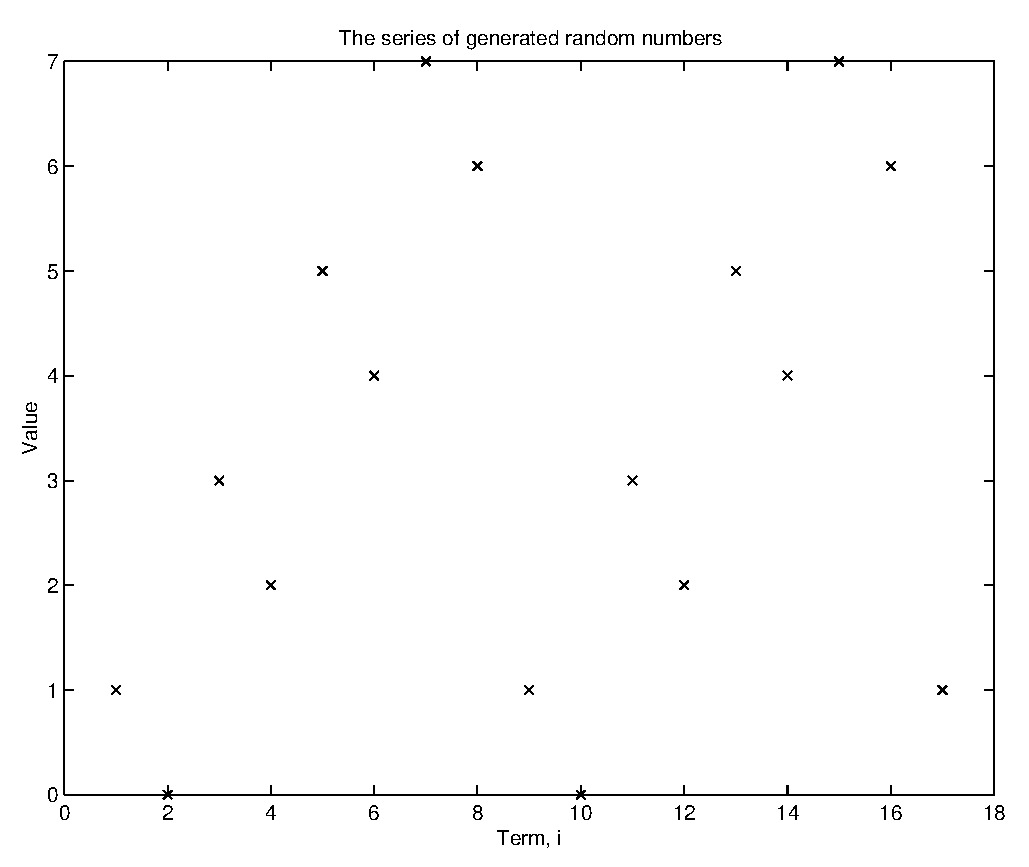
\includegraphics[width=10cm]{./Figures/f_trandom1.eps}
\caption{Successive values in a series of random numbers generated
for a=5, c=3, M=8. Note that the even numbers are always one less 
then the odd ones!}
\end{figure}
It might be instructive to run the program keeping the multiplier 
and the modulo fixed while changing the increment. The result of 
these runs are summarized in Table \ref{T_LCG}.

\begin{table}
\label{T_LCG}
\caption{Series of random numbers for the linear congruential 
generator of the form $I_{n+1} = (5I_n +c) \mod 8$}
\begin{tabular}{ccc} \hline
c &  $I_n$ & Period  \\ \hline
1 & 1,6,7,4,5,2,3,0 & 8 \\
2 & 1,7,5,3,1,7,5,3 & 4 \\
  & 4,6,0,2,4,6,0,2 & 4 \\
3 & 1,0,3,2,5,4,7,6 & 8 \\
4 & 1,1,1,1,1,1,1,1 & 1 \\
  & 2,6,2,6,2,6,2,6 & 2 \\
  & 3,3,3,3,3,3,3,3 & 1 \\
  & 4,0,4,0,4,0,4,0 & 2 \\
  & 5,5,5,5,5,5,5,5 & 1 \\
  & 7,7,7,7,7,7,7,7 & 1 \\
5 & 1,2,7,0,5,6,3,4 & 1 \\
6 & 1,3,5,7,1,3,5,7 & 4 \\
  & 2,0,6,4,2,0,6,4 & 4 \\
7 & 1,4,3,6,5,0,7,2 & 8
\end{tabular}
\end{table}
It is evident that a wrong  choice of the constants leads to a 
very poor random sequence.

It can be shown that (Knuth)  that in the case $c=0$ the full 
period, 1 to $M-1$ can be achieved by choosing $M$ as aprime 
number and for $a$, a primitive element modulo $m$, i.e., for all 
prime divisors, $p$, of $(M-1)$, 
\begin{equation*}
a^{(M-1)/p} {\rm mod} M \ne 1.
\end{equation*}
For the case of $c\ne 0$ the full period is obtained if the 
following three conditions are satisfied:

(i) $c$ and $M$ are relatively prime,

(ii) $a {\rm mod} p = 1$ for each prime factor $p$ of $M$,

(iii) $a {\rm mod} 4 = 1$ if 4 divides $M$.

It is evident that the greater the modulus the longer the period.
For example the MATLAB random number generating function uses
\begin{equation*}
a= 16807; c=0; M=2^{31}-1.
\end{equation*}
This chioce has been suggested by Park and Miller (Lit. Press).
The period of the generator is $2^{31}-2 \approx 2.1 \times 10^9$.
Another poupular popular random generator uses
\begin{equation*}
a= 65539; M=2^{31}-1; c=0,
\end{equation*}
and will be used in the following program {\sf trandom2.m}. There 
we will draw a number $n=xxx$ of random numbers using the linear 
congruential method. In the program we will check the quality of 
the generator by plotting the 1D, 2D, and 3D distribution of the 
pseudo--random numbers. The results of the test can be seen in 
Figs. (\ref{F_TRANDOM2_1}), (\ref{F_TRANDOM2_2}), 
(\ref{F_TRANDOM2_3}), and (\ref{F_TRANDOM2_4}).



\subsubsection{Listing of the program trandom2.m}
\begin{verbatim}
% trandom2 - Program to test random number generators
% The program makes use of the random number generator random1
clear; help trandom2; % clear memory and print header
% Enter dimension of random vector
n= input('Enter value of n-'); % 
% generate random vector
R1=random1(n);
% plot random vector
plot(R1)
title('random numbers'); xlabel('random variable');
disp('Histogram: press any keyboard key');
pause;
% plot histogram of random numbers
x=(0.05:0.1:0.95);
[m,xout] = hist(R1,x);
bar(xout,m)
xlabel('random number');
title('1D distribution: Histogram');
disp('2D plot: press any keyboard key');
pause;
% 2D plot: correlation of consecutive numbers
R2x=R1(1:2:n-1);
R2y=R1(2:2:n);
plot(R2x,R2y,'x')
title('2d distribution')
disp('3D plot: press any keyboard key');
pause;
% 3D plot: correlation of consecutive numbers
R3x=R1(1:3:n);
R3y=R1(2:3:n);
R3z=R1(3:3:n);
%R3=random1(n,3);
plot3(R3x,R3y,R3z,'x')
title('3D distribution');xlabel('Random number');
\end{verbatim}

\subsubsection{Listing of the function {\sf random1}}
%%%%%%%%%%%%%%%%%%%%%%%%%%%%%%%%%%%%%%%%%%%%
\begin{verbatim}
function R = random1(n)
% function to generate random numbers
a=65539;
M=2^(31)-1;
R(1) = 12345678;
for j=1:n-1
%   for i=1:n-1
   R(j+1) =floor(rem(a*R(j),M));
%end
end
R=R/M;
\end{verbatim}

\begin{figure}
\label{F_TRANDOM2_1}
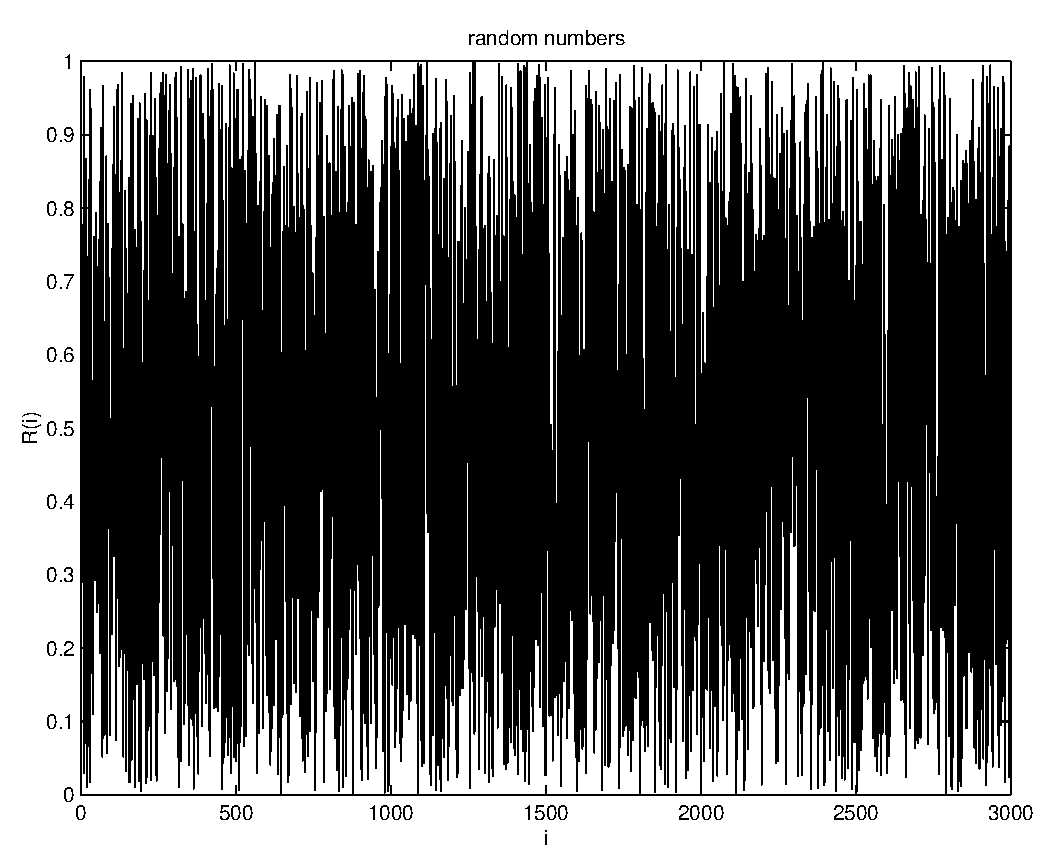
\includegraphics[width=10cm]{./Figures/f_trandom2_1.eps}
\caption{Successive values in a series of 3000 random numbers generated
for $a=65539$, $c=0$, $M=2^{31}-1$.}
\end{figure}

\begin{figure}
\label{F_TRANDOM2_2}
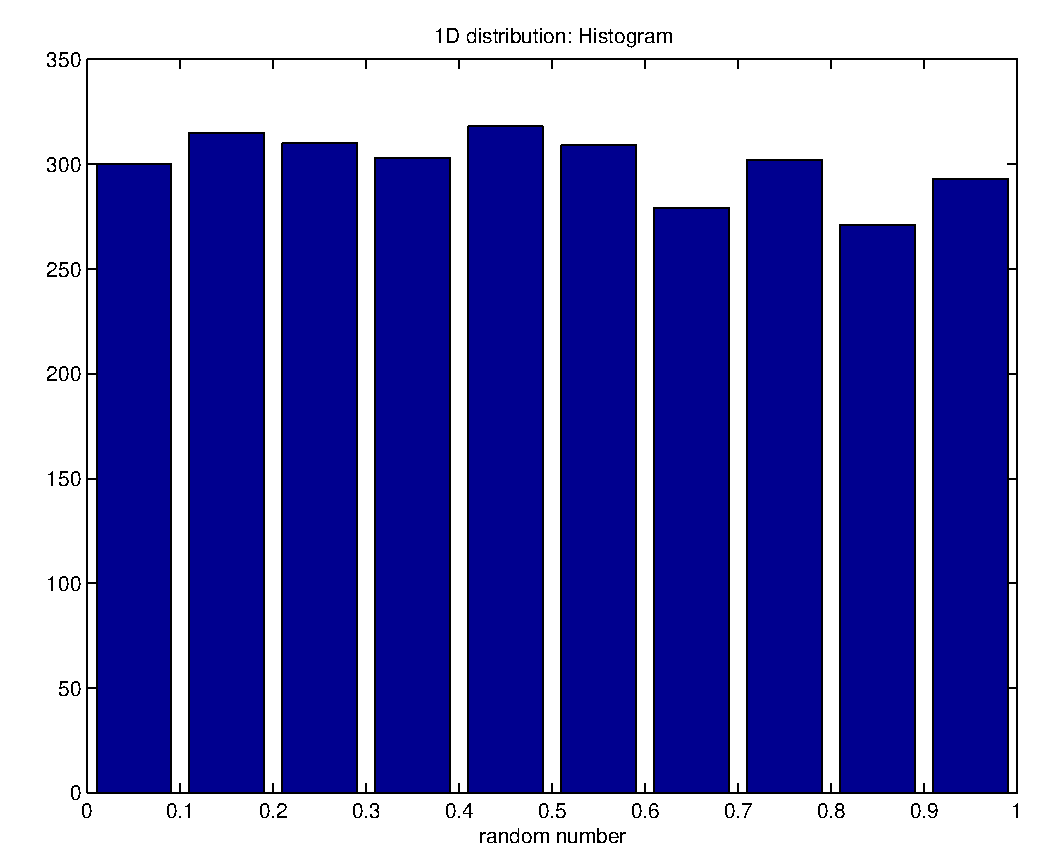
\includegraphics[width=10cm]{./Figures/f_trandom2_2.eps}
\caption{Histogram for a series of 3000 random numbers generated
for $a=65539$, $c=0$, $M=2^{31}-1$.}
\end{figure}

\begin{figure}
\label{F_TRANDOM2_3}
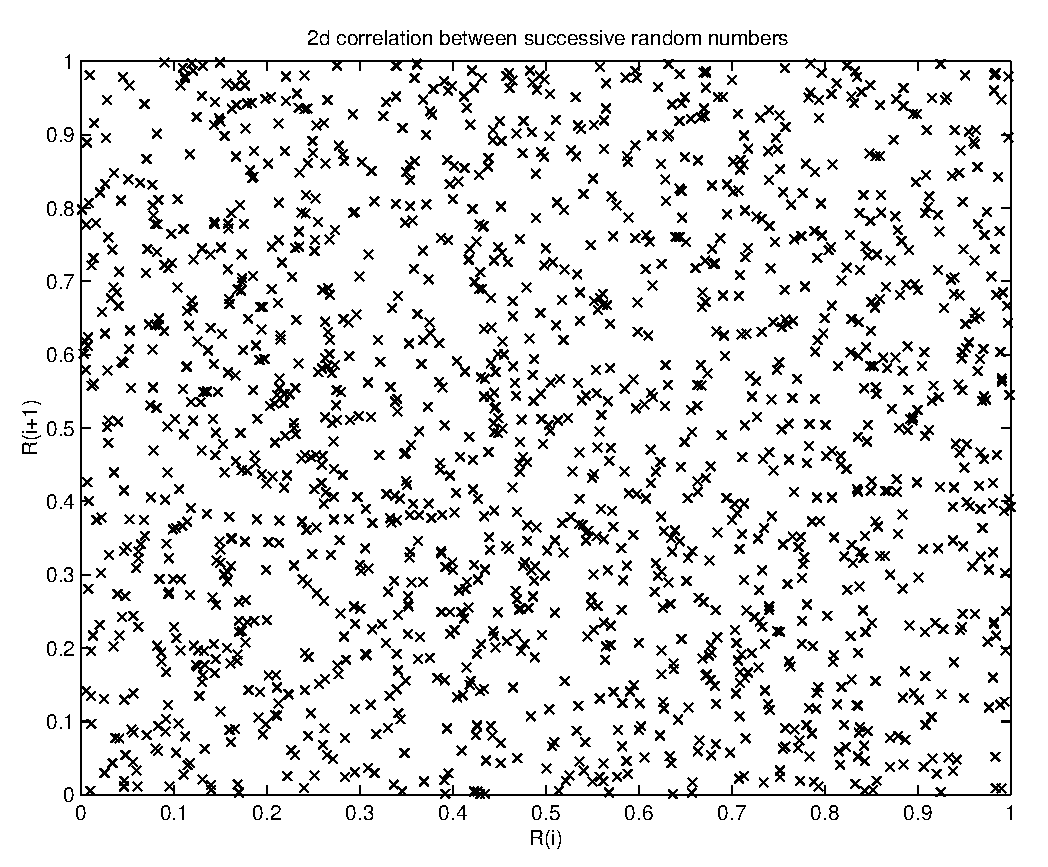
\includegraphics[width=10cm]{./Figures/f_trandom2_3.eps}
\caption{Correlation between successive values in a series of 3000 
random numbers generated for $a=65539$, $c=0$, $M=2^{31}-1$.}
\end{figure}


\begin{figure}
\label{F_TRANDOM2_4}
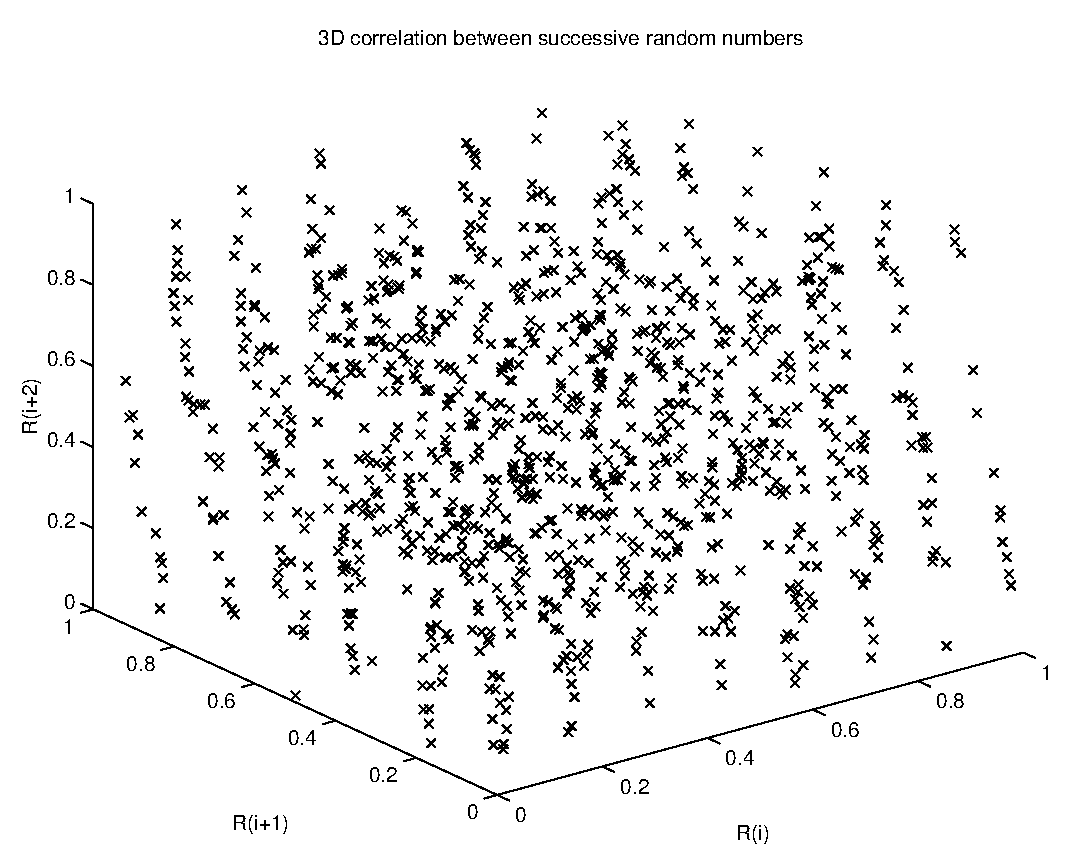
\includegraphics[width=10cm]{./Figures/f_trandom2_4.eps}
\caption{Correlation between successive values 
$R(i),R(i+1), R(i+2)$ in a series of 3000 random numbers generated
for $a=65539, c=0, M=2^{31}-1$.}
\end{figure}

The figures clearly reveal that the generator is not perfect.
In the exercise we will learn that choosing $a=16807$, the minimal
standard generator, 
significantly improves the performance. The performance of 
this minimal standard generator can be increased by shuffling
the output to remove low--order serial correlations (EXERCISE!!!!)
({\sf ran1} of Numerical Recipes).

In the book by Press et al. other "Quick and Dirty" linear 
congruential generators
are presented. Furthemore, serial correlations can be broken up by 
combining two linear congruential generators.

There are also other algorithms for the generation of random 
numbers: Shift--register generators (Lit: Kirkpatrick and Stoll), 
Fibonacci generators (lit: Knuth, James) or quasi--random numbers 
and we refer the reader to the original literature.

\section{The Transfomation method: Invertible distributions}
In the previous section we have learned how to generate random 
numbers with a uniform probability distribution, so that the 
probability $p(x)dx$ to generate a random number between $x$ and $x+dx$
is given by
\begin{equation*}
P(x)dx = \left\{ \begin{array}{ll}
                   dx & 0<x<1 \\
                   0   & {\rm otherwise}.
                  \end{array}
         \right.
\end{equation*}
With the help of the random variable transformation theorem it is easy
to transform uniform deviates into random numbers which are 
distributed according to invertible, one--to--one, distributions.
We know from Chap. 2 that if we take a uniform deviate $x$ and then 
transform it to a new variable $y(x)$ the probability distribtion
of $y$ is given by
\begin{equation}
p(y) = p(x) \left| \frac{dx}{dx}\right|.
\end{equation}
We want to derive a transformation which generates random numbers 
which are distributed according to a given
$p(y)$. Since $x$ is uniformly distributed the 
above equation reduces to
\begin{equation}
\label{INVERTIBLE}
\frac{dx}{dy} = p(y),
\end{equation}
which can be easily integrated
\begin{equation*}
x(y) = P(y) = \int^y p(y')dy'.
\end{equation*}
Hence, the transformation we are looking for is given by the 
inverse of $P(y)$. Thus, a random variable $Y$ with density $p(y)$
can be generated by uniform deviates trough
\begin{equation*}
Y = Y(X) = P^{-1}(X).
\end{equation*}
In the following we will apply this method to generate 
exponentially and gaussian distributed random numbers.

\subsection{Exponential distribution}
Let $p(y)= w\exp(-wy)$ for positive $y$. It follows from Eq. (\ref{INVERTIBLE})
that
\begin{equation*}
\frac{dx}{dy} = w \exp(-wy).
\end{equation*}
Therefore we get immediately
\begin{equation*}
x(y) = \int_0^{\infty} dy'w\exp(-wy') = 1-\exp(-wy).
\end{equation*}
The above expression is easily inverted
\begin{equation*}
y=-\frac{1}{w}\ln(1-x),
\end{equation*}
and since $x$ is equally distributed in $[0,1]$ we can generate 
exponentially distributed random numbers with the help of the 
formula
\begin{equation}
y = - \frac{1}{w} \ln(x).
\end{equation}
It is clear that in MATLAB such an exponentially distributed 
random number $Y$ can be generated with the help of the following 
line of code
\begin{verbatim}
y = - log( rand(1) )/w
\end{verbatim}
With the help of the simple program {\sf expdistr} we want to 
generate 1000 exponentially distributed random numbers and compare
them with the prescribed distribution. We check also the mean 
value and variance and compare them with the analytical expectation 
values.

\subsubsection{Listing of the program expdistr.m}

In Fig. (\ref{F_EXPDISTR}) we see the histogram of 1000 drawn exponentially 
distributed random numbers.
\begin{figure}
\label{F_EXPDISTR}
\includegraphics[width=10cm]{./Figures/f_expdistr.eps}
\caption{Histogram of 1000 exponentially distributed random numbers with
mean 1 generated according to the transformation method. The continuous
line represents the expected exponential distribution.}
\end{figure}

\subsection{Gaussian distributed random numbers}
Gaussian distributed random numbers can be obtained with the help 
of the multidimensional random variable transformation theorem.
Let us consider the transformation
\begin{eqnarray}
\label{GAUSS-GEN1}
y_1 & = & \sqrt{-2\log(x_1)} \cos(2 \pi x_2) \\
\label{GAUSS_GEN2}
y_2 & = & \sqrt{-2\log(x_1)} \sin(2 \pi x_2),
\end{eqnarray}
where $X_1$ and $X_2$ are uniformly distributed random numbers on 
the interval $[0,1)$. Equivalently we can write
\begin{eqnarray*}
x_1 & = & \exp[-\frac{1}{2}(y_1^2+y_2^2)] \\
x_2 & = & \frac{1}{2 \pi} \arctan\left( \frac{y_1}{y_2}\right).
\end{eqnarray*}
it is now straightforward  to show that the Jacobian determinant
reads
\begin{equation*}
\frac{\partial(x_1,x_2)}{\partial(y_1,y_2)} = 
   - \left[ \frac{1}{\sqrt{2 \pi}} \exp(-y_1^2/2)\right]
   \left[ \frac{1}{\sqrt{2 \pi}} \exp(-y_2^2/2)\right].
\end{equation*}
The right hand side of the above equation corresponds to the 
product of two independent Gaussian distributions. Thus it follows
from the multidimensional version of the random variable 
transformation  theorem for invertible distributions that the
two random number generated according to Eqs. (\ref{GAUSS-GEN1}) 
and (\ref{GAUSS-GEN2}) are Gaussian distributed. This algorithm 
which allows the generation of two Gaussian random numbers from 
two uniformly distributed ones is called the Box--Muller method.

It is clear that it easy to implement the above algorithm in 
MATLAB. This is done in the program {\sf gaussdistr.m} which generates
gaussian random numbers with mean value $mu$ and variance $sigma$.

\subsubsection{Listing of the program gaussdistr.m}

The corresponding histogram obtained by running the program for
n=1000, mu=0, sigma=2 can be seen in Fig. (\ref{F_GAUSSDISTR}).
\begin{figure}
\label{F_GAUSSDISTR}
\includegraphics[width=10cm]{./Figures/f_gaussdistr.eps}
\caption{Histogram of 1000 Gaussian distributed random numbers with
mean 0 and variance 2 generated according to the Box-Muller method. 
The continuous line represents the expected Gaussian density.}
\end{figure}

Let us end this subsection by mentioned that normal distributed
random numbers can be generated in MATLAB with the help of 
the function {\sf randn}.

\section{The acceptance--rejection technique}
The acceptance--rejection technique is a method of wide 
applicability. In its original formulation it is due to 
von--Neumann. The basic idea is to sample a random number
from some known and appropriate probability distribution and to 
perform a test to determine whether or not it is acceptable for 
use or not. We follow Rubinstein but consider for simplicity only
the one--dimensional case.

Let us assume that the stochastic variable $X$ is defined on the 
interval $a \le x \le b$ and is distributed according to the
probability density $p(x)$. We write this probability distribution 
as
\begin{equation*}
p(x) = C d(x) q(x),
\end{equation*}
where $C$ is a normalization constant $C \ge 1$, $q(x)$ is also a 
probability distribution and $0 \le d(x) \le 1$. The probability 
distribution $q(x)$ is the importance function, and  we are 
supposed to know how to generate random variates distrubuted 
according to it.

The accepatnce--rejection method works as follows. We generate two
random variates, $\xi$ is uniformly distributed on the interval
$[0,1)$ and $Y$ is distributed according to $q(y)$. Then we test
whether or nor the equality
\begin{equation*}
\xi \le d(y)
\end{equation*}
holds or not. If  the conditione $\xi \le d(y)$ is satisfied, 
then $Y$ is accepted as 
a random variate distributed according to $p(x)$.  If
the condition is not satisfied, the pair $(\xi,y)$ is rejected, 
and we have to try again.

It is easy to demonstrate that the above methd works. Let us apply
Bayes'formula to the conditional probability $p(x|\xi \le d(y)$:
\begin{equation}
\label{A-R-BAYES}
p(x|\xi \le d(y) = \frac{{\rm Prob}(p(x|\xi \le d(y)|Y=x)q(x)}
                  {{\rm Prob}(\xi \le d(y))}.
\end{equation}
It is straightforward to compute
\begin{eqnarray*}
{\rm Prob}(p(x|\xi \le d(y)|Y=x) &=& {\rm Prob}(\xi \le d(x)) = 
          d(x) \\
{\rm Prob}(\xi \le d(y)) & = & \int {\rm Prob}(\xi \le d(Y|Y=x)) q(x) dx \\
               &= & \int q(x) d(x)dx = \int dx \frac{p(x)}{C} = 
                   \frac{1}{C}.
\end{eqnarray*}
Inserting into (\ref{A-R-BAYES}) we obatin finally
\begin{equation*}
p(x|\xi \le d(y) = p(x),
\end{equation*}
which completes the proof.

The above discussion also makes evident the role of the constant
$C$. The efficiency of the method depends on the inequality $\xi \le 
d(y)$, for independent trials the probability of success is given 
by $1/C$. $C$ represents the average number of passes which must 
be made with the algorithm in order to select a variate. It is 
clear, that in order for the method to be efficient it must be 
easy to generate random numbers according to $q(x)$ and the 
efficiency should be large, i.e., $C$ should be close to one.

In the original formulation by von--Neumann the comparison 
function was simply chosen to be the uniform distribution. If
$M$ is the maximum of $p(x)$ then we choose
\begin{eqnarray*}
q(x) & = & \frac{1}{b-a} \\
d(x) & = & \frac{p(x)}{M} \\
C & = & M(b-a).
\end{eqnarray*}
The von--Neumann algorithm then simply reads \\
1. Generate $\chi_1$ and $\chi_2$ uniformly distributed in 
    $[0,1)$. \\
2. Evaluate $Y=a+\chi_2(b-a)$. \\
3. If $\chi_1 \le p(x)/M$ then $Y$ is a variate distributed 
    according to $p(x)$. \\
4. Go to 1.

As a simple example we want to generate random numbers on $[0,1)$    
distributed according to
\begin{equation*}
p(x) = 3x^2; \;\;\; 0 \le x <1.
\end{equation*}
We choose $C=3$ and apply the von--Neumann algorithm. \\
1. Generate $\chi_1$ and $\chi_2$ uniformly distributed in 
    $[0,1)$. \\
2. Test the inequality $\chi_1 \le \chi_2^2.$     \\
3. If the equality holds we accept $\chi_2$ as a random number 
generated according to $p(x)$.

The above algorithm has been implemented in MATLAB in the program
{\sf neumann.m}, which we run for $n=1000$ and $n=5000$. The 
result of the latter run can be seen in Fig. (\ref{F_NEUMANN}).
\begin{figure}
\label{F_NEUMANN}
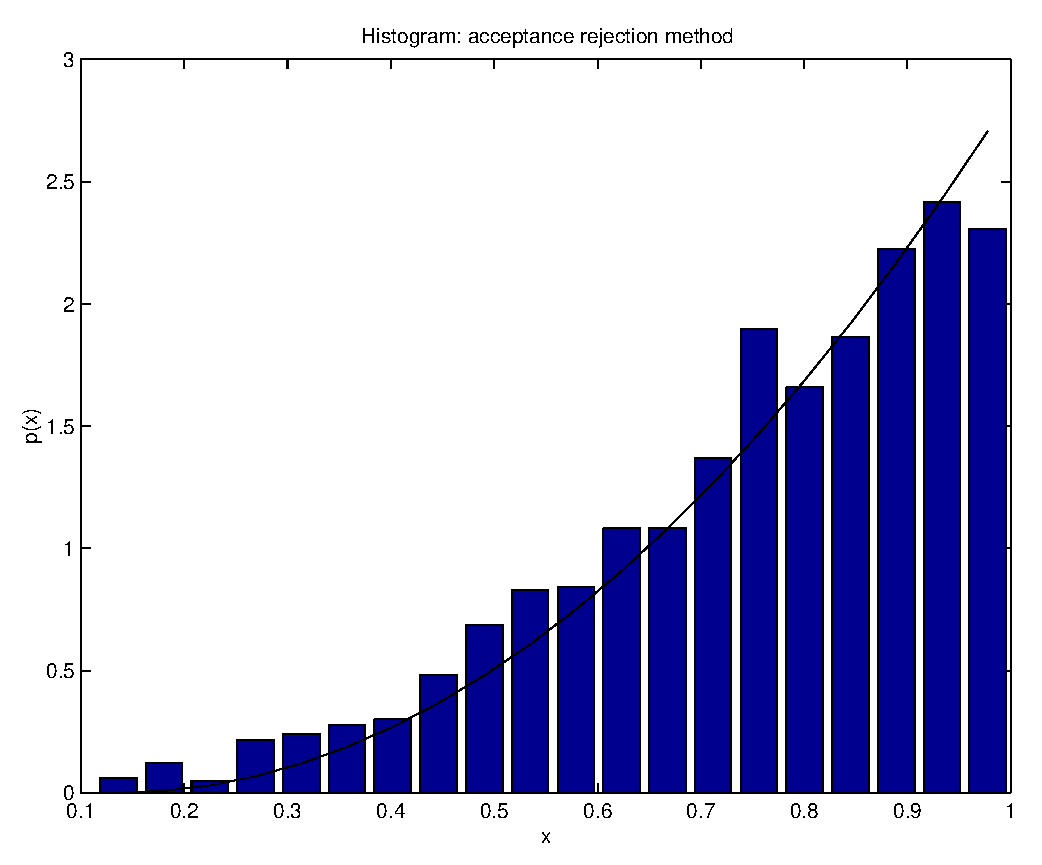
\includegraphics[width=10cm]{./Figures/f_neumann.eps}
\caption{Histogram of 5000 random numbers distributed
according to $p(x) = 3x^2$ generated with the von--Neumann
acceptance--rejection technique.
The continuous line represents the exact density $p(x)$.}
\end{figure}
In the program we count the number of successful trials. The ratio
of successful trials to the total number of drawn random pairs for 
the run shown
is 0.3328, which is in good agreement we the expected theoretical
value of $1/C=1/3$.

\subsubsection{Listing of the program neumann.m}




%\subsection{Poisson distributed random numbers}

\section{Variance reduction: Importance Sampling}
In this section we will see how the Monte--Carlo integration
algorithms can considerably be improved. The importance sampling 
technique will be our first encounter with a so--called variance 
reduction technique. We already know that the estimation of 
integrals by the Monte--Carlo method is affected with errors. The
basic idea of variance reduction techniques is to use known 
informations about the problem in order to improve the efficiency 
of the simulation. Obviuosly, if nothing is known about the 
problem no variance reduction can be achieved. On the other 
extreme, if we have full knowledge the variance will be reduced to 
zero, and there will be no need for a simulation. It is always 
important to be aware of what is known about the system.

We now consider the problem of estimating the integral
\begin{equation}
\label{INT_VARRED}
I = \int dx f(x).
\end{equation}
The central idea of importance sampling is to select random 
variates from regions in proportion to the importance these 
regions make to the integral we want to evaluate, instead of 
spreading them evenly. To this end we rewite the integral 
(\ref{INT_VARRED}) in the form
\begin{equation*}
I = \int \frac{f(x)}{p(x)} p(x) dx = \langle 
\frac{f(x)}{p(x)}\rangle,
\end{equation*}
where $X$ is a random variable with probability density $p(x)$.
$P(x)$ is called the importance sampling distribution.  Since the
integral is obviously the expectation value of the function $f(x)/p(x)$
it can be estimated using $N$ random numbers $X_i$ distributed 
according to $p(x)$
\begin{equation*}
\hat{I}_N = \frac{1}{N} \sum_{i=1}^N \frac{f(x_i)}{p(x_i)}.
\end{equation*}
The function $p(x)$ has to be chosen in such a way that the 
variance of $f(x)/p(x)$ 
\begin{equation*}
{\rm Var} = \langle (\frac{f(x)}{p(x)}-I)^2\rangle
   = \int_a^b \frac{f^2(x)}{p(x)}dx - I^2
\end{equation*}
is minimal. If $f(x)>0$ it follows from the above equation that
${\rm Var}=0$ if we choose $p(x)$ as $p(x) = f(x)/I$. 
Unfortunately, this choice implies that we have to know already 
the integral we want to solve. In general, the variance can 
essentially be reduced if $p(x)$ is chosen to resemble $f(x)$.

As an example we consider the integral
\begin{equation}
\label{I_MCI_IS}
I= \int_0^1 dx \exp(-x^2).
\end{equation}
In the first two columns of table (\ref{T_MCI_IS}) we show
the results of two estimates of the above integral with the 
help of the standard Monte--Carlo integration. In the third column 
we show the results of the importance sampling integration.

\begin{table}\label{T_MCI_IS}
\caption{Monte--Carlo estimates of the integral (\ref{I_MCI_IS})
using the standard method $p(x)=1$ and the importance sampling method
$p(x)=a\exp(-x)$}
\begin{center}
\begin{tabular}{llll}
 ~             & $p(x) =1$ & $p(x) =1$ & $p(x)=a\exp(-x)$ \\ \hline
$N$            & 1000      & 16384      & 1000           \\
$I$            & 0.736087  & 0.74504    & 0.748340        \\
$\sigma_I$     & 0.00131   & 0.000317   & $9.65 \times 10^{-5}$ \\
CPU time/trial (s) & 0.000660  & 0.003837   & 0.000860  \\
total CPU time (s) & 0.66      & 62.86      & 0.86 
\end{tabular}
\end{center}
\end{table}
The simulation was performed with the help of the program
{\sf mciis.m} whose listing can be seen below.

\subsubsection{Listing of the program mciis.m}
%\includelistings{.\Listings\mciis.m}

The importance sampling function is chosen to be $p(x)=a\exp(-x)$,
where the constant $a$ is chosen such that $p(x)$ is normalized
on the  unit interval. Accordingly the $N$ random numbers $X_i$
distributed according to $p(x)$ are generated with the help of the
inversion method. Since
\begin{equation*}
P(x) = \int_0^x dx' p(x') = a[1-\exp(-1)]
\end{equation*}
the exponentially distributed random numbers on the interval $[0,1)$
are generated according to
\begin{equation*}
X = - \log(1- \chi/a),
\end{equation*}
where the $chi$ are uniformly distributed random numbers on the 
interval $[0,1)$. The generation of these random numbers is 
performed in lines x to y.

It is important to remark that although the computation time per
trial is larger in the importance sampling technique the total CPU 
time is smaller compared to the standard Monte Carlo algorithm 
because a much smaller number of realizations is required in order
to achieve a desired accuracy (variance).





\section{Self--Avoiding random walks}
\subsection{Simple sampling}
\subsection{Importance sampling}
%%%%%%%%%%%%%%%%%%%%%%%%%%%%%%%%%%%%%%%%%%%%%%%%%%%%
%%%%%%%%%%%%%%%%%%%%%%%%%%%%%%%%%%%%%%%%%%%%%%%%%%%%%
%%%%%%%%%%%%%%%%%%%%%%%%%%%%%%%%%%%%%%%%%%%%%%%%%%%%%
%%%%%%%%%%%%%%%%%%%%%%%%%%%%%%%%%%%%%%%%%%%%%%%%%%%%%
%%%%%%%%%%%%%%%%%%%%%%%%%%%%%%%%%%%%%%%%%%%%%%%%%%%%%
%%%%%%%%%%%%%%%%%%%%%%%%%%%%%%%%%%%%%%%%%%%%%%%%%%%%%
%%%%%%%%%%%%%%%%%%%%%%%%%%%%%%%%%%%%%%%%%%%%%%%%%%%%%
\chapter{Stochastische Prozesse}
Master-Gleichungen

\chapter{Monte Carlo Methoden in der statistischen Mechanik}
Metropolis; Ising; Finite-Size Effects; Random Walks; SAW (?)
Simulated annealing; travelling salesman;

\chapter{Non-equilibrium MC}
Chemische Reaktionen, Diffusion; Reaktions-Diffusion, Turbulenz.

\chapter{Brownsche Dynamik Simulationen}
Omega-entwicklung; SDE;


\chapter{Rest}
stochastische Resonanzen; Muster Erkennung; random Walks;

\chapter{Stochastische Wellenfunktionsmethoden}
